%Autor: Simon Walker
%Version: 1.0
%Datum: 09.06.2020
%Lizenz: CC BY-NC-SA

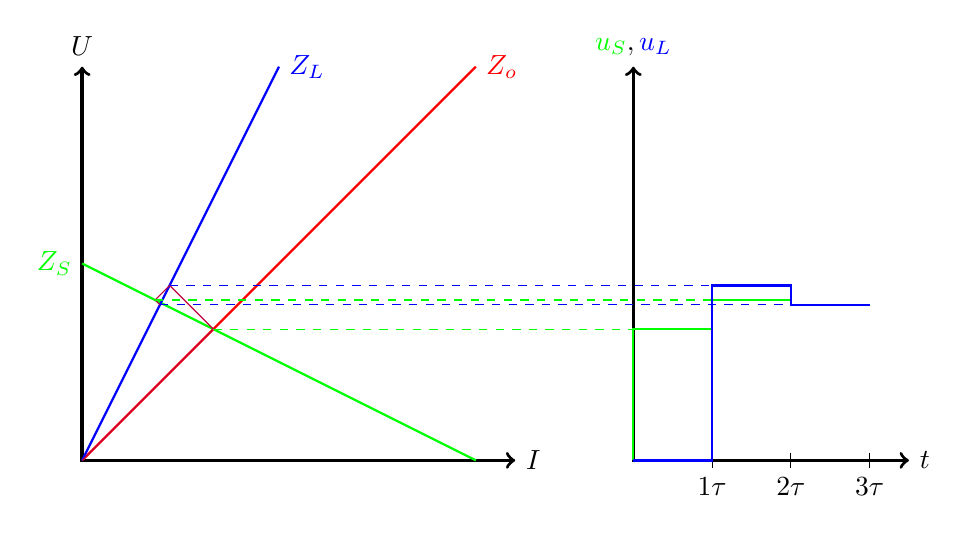
\begin{tikzpicture}
	%\HelpCords{0}{0}{12}{6}
	%Achsen
	\draw[very thick, <->]
	(0,5) node[above] {$U$} -- (0,0) -- (5.5,0)
	node[right] {$I$};
	
	\draw[very thick, <->]
	(7,5) node[above] {$\color{green} u_S \color{black}, \color{blue} u_L$} -- (7,0) -- (10.5,0)
	node[right] {$t$};
	
	%Beschriftung t-Achse
	\draw (8, 0.1) -- (8, -0.1) node[below]	{$1\tau$};
	\draw (9, 0.1) -- (9, -0.1) node[below]	{$2\tau$};
	\draw (10, 0.1) -- (10, -0.1) node[below] {$3\tau$};

	
	%Z_S
	\draw[thick, green] (0, 2.5) node[left, green] {$Z_S$} -- (5, 0); %yS=-0.5x+2.5
	
	%Z_0
	\draw[thick, red] (0, 0) -- (5, 5) node[right, red] {$Z_o$}; %y0=x
	
	%Z_L
	\draw[thick, blue] (0, 0) -- (2.5, 5) node[right, blue] {$Z_L$}; %yL=2x
	
	%Welle
	%Berechnungen
	%SP1: yS=y0 (1.6666, 1.6666) 
	%SP1-SP2 y1=-x+3.3333
	%SP2: yL=y1 (1.1111, 2.2222)
	%SP2--SP3 y2=x+1.1111
	%SP3: yS=y2 (0.9259, 2.0370)
	%SP3--SP4 y3=-x+2.9629
	%SP4: yL=y3 (0.9876, 1.9752)
	
	\draw[purple] (0,0) -- (1.6666, 1.6666) -- (1.1111, 2.2222) -- (0.9259, 2.0370) -- (0.9876, 1.9752);
	
	%t=0
	\draw[dashed, green] (1.6666, 1.6666) -- (7, 1.6666);
	
	%t=1tau
	\draw[dashed, blue] (1.1111, 2.2222) -- (8, 2.2222);
	
	%t=2tau
	\draw[dashed, green] (0.9259, 2.0370) -- (9, 2.0370);
	
	%t=3tau
	\draw[dashed, blue] (0.9876, 1.9752) -- (10, 1.9752);
	
	%u_S
	\draw[thick, green] (7, 0) -- (7, 1.6666) -- (8, 1.6666) -- (8, 2.0370) -- (9, 2.0370);
	\draw[thick, blue] (7, 0) --(8, 0) -- (8, 2.2222) -- (9, 2.2222) -- (9, 1.9752) -- (10, 1.9752);
	
	
		
\end{tikzpicture}
